%%===================================================================
%% Lecture 17 -- The Higgs Mechanism in Unitary Gauge and the Lepton Standard Model
%% 77609 -- Introduction to Elementary Particles
%% Date: 11/06/2026
%% Lecturer: Prof. Yonit Hochberg
%%===================================================================

\section{Lecture 17 -- The Higgs Mechanism in Unitary Gauge and the Lepton Standard Model}\label{sec:lec17}
\begin{center}
\begin{tabular}{ll}
  \textbf{Date:}\quad 11/06/2026 & \\
\end{tabular}
\end{center}
\hrule\vspace{1.5em}

%%------------------------------------------------------------------
\subsection{Overview}\label{subsec:lec17:overview}

Lecture~16 stated the Higgs mechanism and introduced the nonlinear (magnitude--phase) realization of a condensing complex scalar. Today we finish that calculation and then put it to work:

\begin{enumerate}
  \item \textbf{The Abelian Higgs model, completed}: in the unitary gauge the would-be Goldstone disappears from the Lagrangian, the gauge boson acquires the mass $m_V^2=g^2v^2$, and the physical spectrum --- one massive vector plus one massive scalar (the Higgs boson) --- is read off directly.
  \item \textbf{General lessons}: gauge bosons of broken generators become massive, gauge bosons of unbroken generators stay massless (protected by the surviving symmetry), and the field that condenses must be a scalar.
  \item \textbf{Fermion masses}: the same vacuum expectation value (vev) gives chiral fermions a mass through Yukawa couplings, exactly as in the global case.
  \item \textbf{The Lepton Standard Model (LSM)}: a complete gauge theory with local $SU(2)_L\times U(1)_Y$ broken spontaneously to $U(1)_{\rm EM}$. We specify its field content, build its Lagrangian piece by piece, identify the unbroken electric-charge generator $Q=T^3+Y$, and begin extracting the gauge-boson mass matrix.
\end{enumerate}

This is the first time all the ingredients of the course --- gauge invariance, representations, chiral fermions, Yukawa couplings, and SSB --- assemble into (a sector of) the actual Standard Model.

%%==================================================================
\subsection{\texorpdfstring{The Abelian Higgs Model in Unitary Gauge}{The Abelian Higgs Model in Unitary Gauge}}\label{subsec:lec17:abelian-higgs}

\subsubsection*{Mathematical Setup}

We return to the theory of Lecture~16: a complex scalar $\phi$ of charge $+1$ under a \emph{local} $U(1)$, with transformation parameter $\theta(x)$ now a function of spacetime,
\begin{equation}
  \phi(x)\to e^{\,i\theta(x)}\phi(x) .
  \label{eq:lec17:u1_transformation}
\end{equation}
The gauge-invariant Lagrangian contains the covariant kinetic term for $\phi$, the kinetic term for the gauge field $A_\mu$, and the symmetry-breaking potential:
\begin{equation}
  \Lag
  =(D_\mu\phi)^\dagger D^\mu\phi
   -\frac14 F_{\mu\nu}F^{\mu\nu}
   -\mu^2\,\phi^\dagger\phi
   -\lambda\,(\phi^\dagger\phi)^2 ,
  \qquad
  D_\mu\phi=(\partial_\mu+i g A_\mu)\phi ,
  \label{eq:lec17:abelian_lagrangian}
\end{equation}
where $g$ is the gauge coupling, $F_{\mu\nu}=\partial_\mu A_\nu-\partial_\nu A_\mu$ is the Abelian field strength, and the charge $+1$ of $\phi$ is already absorbed into $D_\mu$. As always we study the region $\mu^2<0$, where the scalar condenses,
\begin{equation}
  |\langle\phi\rangle|=\frac{v}{\sqrt2},
  \qquad
  v^2=-\frac{\mu^2}{\lambda}>0 ,
  \label{eq:lec17:vev}
\end{equation}
and we choose the real component of $\phi$ to carry the vev. Instead of splitting $\phi$ into real and imaginary parts (the linear realization), we use the \emph{nonlinear realization} in magnitude--phase variables,
\begin{equation}
  \phi(x)=e^{\,i\chi(x)/v}\,\frac{v+h(x)}{\sqrt2} ,
  \label{eq:lec17:nonlinear}
\end{equation}
with $h$ the radial excitation and $\chi$ the phase (would-be Goldstone) excitation, both with vanishing vev. To leading order this agrees with the linear realization, as verified in the homework.

\subsubsection*{The Unitary Gauge Choice}

The original $U(1)$ is spontaneously broken, so the transformation \eqref{eq:lec17:u1_transformation} is no longer a symmetry of the vacuum --- but it is still a valid \emph{change of basis} of our description, and we may pick whichever basis is most convenient. Choose the gauge parameter to cancel the phase of $\phi$ point by point:
\begin{equation}
  \boxed{\;\theta(x)=-\frac{\chi(x)}{v}\qquad(\text{unitary gauge})\;.}
  \label{eq:lec17:unitary_gauge_choice}
\end{equation}

\textit{Significance:} Because the symmetry is local, the phase $\chi(x)$ can be rotated away \emph{everywhere}, something no global transformation could do --- this is precisely the freedom that lets the gauge field eat the Goldstone.

Under this transformation the fields become
\begin{equation}
  \phi\ \to\ \phi'=\frac{v+h(x)}{\sqrt2},
  \qquad
  A_\mu\ \to\ V_\mu= A_\mu+\frac{1}{gv}\,\partial_\mu\chi ,
  \label{eq:lec17:unitary_fields}
\end{equation}
where the shift of the gauge field follows from the usual gauge transformation $A_\mu\to A_\mu-\tfrac1g\partial_\mu\theta$ with $\theta=-\chi/v$. The phase $\chi$ has not been deleted; it has been moved into the gauge field $V_\mu$.

\subsubsection*{Expanding the Lagrangian}

Insert the unitary-gauge fields \eqref{eq:lec17:unitary_fields} into \eqref{eq:lec17:abelian_lagrangian}. The covariant derivative acts on a now-real field,
\begin{equation}
  D_\mu\phi'
  =\big(\partial_\mu+i g V_\mu\big)\frac{v+h}{\sqrt2}
  =\frac{1}{\sqrt2}\,\partial_\mu h+\frac{i g}{\sqrt2}\,V_\mu\,(v+h) ,
  \label{eq:lec17:Dmu_unitary}
\end{equation}
so its modulus squared is
\begin{equation}
  (D_\mu\phi')^\dagger D^\mu\phi'
  =\frac12\,\partial_\mu h\,\partial^\mu h
  +\frac{g^2}{2}\,V_\mu V^\mu\,(v+h)^2 .
  \label{eq:lec17:kinetic_expanded}
\end{equation}
For the potential, write it in the shifted form $V(\phi)=\lambda\big(\phi^\dagger\phi-\tfrac{v^2}{2}\big)^2$ (equal to the original up to a constant). With $\phi^\dagger\phi=\tfrac12(v+h)^2$,
\begin{equation}
  \phi^\dagger\phi-\frac{v^2}{2}=v h+\frac{h^2}{2}
  \quad\Longrightarrow\quad
  V=\lambda\Big(v h+\frac{h^2}{2}\Big)^2
  =\lambda v^2 h^2+\lambda v\,h^3+\frac{\lambda}{4}h^4 .
  \label{eq:lec17:potential_expanded}
\end{equation}
Expanding $(v+h)^2=v^2+2vh+h^2$ in \eqref{eq:lec17:kinetic_expanded} and collecting everything:
\begin{equation}
  \boxed{\;
  \Lag=-\frac14 F_{\mu\nu}F^{\mu\nu}
  +\frac12\,\partial_\mu h\,\partial^\mu h
  +\frac12 g^2v^2\,V_\mu V^\mu
  -\frac12\big(2\lambda v^2\big)h^2
  +\frac{g^2}{2}V_\mu V^\mu\,h\,(2v+h)
  -\lambda v\,h^3-\frac{\lambda}{4}h^4
  \;}
  \label{eq:lec17:unitary_lagrangian}
\end{equation}
where $F_{\mu\nu}$ is now built from $V_\mu$. Note what is absent: the field $\chi$ appears nowhere.

\textit{Significance:} Written around the true vacuum in unitary gauge, the Lagrangian displays the physical particle content directly --- every field that appears is a physical excitation, with its mass and interactions in plain sight.

\subsubsection*{The Physical Spectrum}

Reading off the quadratic terms of \eqref{eq:lec17:unitary_lagrangian}: the term $\tfrac12 g^2v^2V_\mu V^\mu$ is a mass term for a real vector ($\tfrac12 m_V^2 V_\mu V^\mu$), and the term $-\tfrac12(2\lambda v^2)h^2$ is a mass term for a real scalar. The elementary particles of the model are therefore
\begin{equation}
  \boxed{\;
  \text{a massive vector boson } V_\mu:\ \ m_V^2=g^2v^2 ,
  \qquad
  \text{a massive scalar } h:\ \ m_h^2=2\lambda v^2 .
  \;}
  \label{eq:lec17:spectrum}
\end{equation}

\textit{Significance:} A gauge boson, whose mass term is forbidden by gauge invariance, has become massive --- possible only because the vacuum, not the Lagrangian, broke the symmetry; both masses vanish as $v\to0$, confirming that the vev is their sole source.

\paragraph{Where did $\chi$ go?}
The field $\chi$ has been \emph{eaten} to give the vector boson its mass. A massless vector has $2$ transverse polarizations; a massive one has $3$. The one degree of freedom of the real scalar $\chi$ has become the longitudinal component of the now-massive $V_\mu$, so the total number of degrees of freedom is unchanged:
\begin{equation}
  \underbrace{2}_{\text{massless }A_\mu}+\underbrace{1}_{\chi}
  =\underbrace{3}_{\text{massive }V_\mu} .
  \label{eq:lec17:dof}
\end{equation}
Choosing the phase to be the eaten degree of freedom is a convenience --- any other parameterization yields the same physics, just less transparently.

\paragraph{Consistency limits.}
\begin{itemize}
  \item $g\to0$: the vector mass $m_V=gv\to0$, and the theory degenerates into a massless gauge boson plus a massless scalar --- the latter is just the Goldstone boson of the global theory. The longitudinal component decouples smoothly.
  \item $v\to0$: no condensate, no SSB, and the gauge boson is massless, exactly as the unbroken symmetry demands. The proportionality of all masses to $v$ is no accident.
\end{itemize}

\dfn[dfn:lec17:higgs-field-boson]{Higgs Field vs.\ Higgs Boson}{
The \emph{Higgs field} is the scalar field $\phi$ that acquires the vacuum expectation value. The \emph{Higgs boson} is the physical particle $h$ --- the radial excitation of the Higgs field around the vacuum, with mass $m_h^2=2\lambda v^2$.
}

\subsubsection*{Parameter Counting and Coupling Relations}

Although the unitary-gauge Lagrangian \eqref{eq:lec17:unitary_lagrangian} contains many interaction terms, they all descend from just \emph{three} independent parameters, e.g.
\begin{equation}
  \boxed{\;\{\lambda,\ v,\ g\}\quad\text{(equivalently }\{\lambda,\mu^2,g\}\text{)}\;.}
  \label{eq:lec17:three_params}
\end{equation}

\textit{Significance:} The absence of an independent coefficient per term --- masses, cubic, and quartic couplings all tied together --- is the experimental fingerprint of spontaneous symmetry breaking.

Two structural features of the interactions deserve emphasis:
\begin{itemize}
  \item \textbf{The $hVV$ coupling is proportional to the gauge-boson mass squared.} The term $g^2v\,V_\mu V^\mu h$ has coefficient $g^2v=m_V^2/v$, so the Higgs couples to the vector in proportion to $m_V^2$:
  \begin{equation}
    \boxed{\;g_{hVV}=g^2v=\frac{m_V^2}{v}\;.}
    \label{eq:lec17:hVV_coupling}
  \end{equation}
  \textit{Significance:} The Higgs boson talks most strongly to the heaviest gauge bosons --- the experimental handle used to discover and study it at the LHC.
  \item \textbf{Dimensionless couplings are unchanged by SSB.} The $h^4$ coefficient ($\lambda/4$) and the $h^2V^2$ coefficient ($g^2/2$) are dimension-four operators with dimensionless coefficients, and they coincide with their values in the symmetric Lagrangian. Only couplings with positive mass dimension are shifted by the vev. This holds for Abelian, non-Abelian, and product-group breaking alike, and is a standard sanity check after any SSB computation.
\end{itemize}

\begin{figure}[ht]
\centering
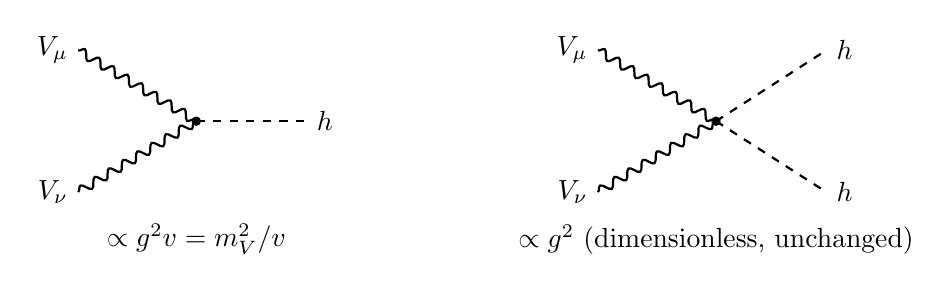
\begin{tikzpicture}[>=stealth,scale=1.0]
  % hVV vertex
  \begin{scope}[xshift=-3.2cm]
    \coordinate (c) at (0,0);
    \draw[decorate,decoration={snake,amplitude=1.6pt,segment length=6pt},thick]
      (-1.5,0.9) node[left]{$V_\mu$} -- (c);
    \draw[decorate,decoration={snake,amplitude=1.6pt,segment length=6pt},thick]
      (-1.5,-0.9) node[left]{$V_\nu$} -- (c);
    \draw[thick,dashed] (c) -- (1.4,0) node[right]{$h$};
    \fill (c) circle (1.7pt);
    \node at (0,-1.5) {$\propto g^2 v=m_V^2/v$};
  \end{scope}
  % hhVV vertex
  \begin{scope}[xshift=3.4cm]
    \coordinate (c) at (0,0);
    \draw[decorate,decoration={snake,amplitude=1.6pt,segment length=6pt},thick]
      (-1.5,0.9) node[left]{$V_\mu$} -- (c);
    \draw[decorate,decoration={snake,amplitude=1.6pt,segment length=6pt},thick]
      (-1.5,-0.9) node[left]{$V_\nu$} -- (c);
    \draw[thick,dashed] (c) -- (1.4,0.9) node[right]{$h$};
    \draw[thick,dashed] (c) -- (1.4,-0.9) node[right]{$h$};
    \fill (c) circle (1.7pt);
    \node at (0,-1.5) {$\propto g^2$ (dimensionless, unchanged)};
  \end{scope}
\end{tikzpicture}
\caption{Higgs--gauge-boson vertices of the unitary-gauge Lagrangian \eqref{eq:lec17:unitary_lagrangian}. Left: the $hVV$ coupling, fixed by the gauge-boson mass, $g_{hVV}=m_V^2/v$. Right: the quartic $hhVV$ coupling, whose dimensionless coefficient $g^2/2$ is inherited unchanged from the symmetric Lagrangian. The cubic $h^3$ and quartic $h^4$ self-couplings ($-\lambda v$ and $-\lambda/4$) complete the interaction list.}
\label{fig:lec17:higgs-vertices}
\end{figure}

\nt{Pitfall: the mass term of a \emph{real} vector field is $+\tfrac12 m_V^2 V_\mu V^\mu$, so from $\tfrac12 g^2v^2 V_\mu V^\mu$ one reads $m_V=gv$ with \emph{no} extra $\sqrt2$. Contrast the fermion mass $m_\psi=yv/\sqrt2$ and the scalar mass $m_h^2=2\lambda v^2$ (not $\lambda v^2$): each spin carries its own normalization, and mixing them up is the most common error in spectrum questions.}

\subsubsection*{Method}

To analyze SSB of a gauge theory and extract its spectrum:
\begin{enumerate}
  \item Identify the gauge group $G$, the matter representations, and write the gauge-invariant Lagrangian with covariant derivatives.
  \item Minimize the potential; record the vev $\langle\phi\rangle$ and the scale $v$.
  \item Test each generator on the vacuum: $T^a\langle\phi\rangle=0$ means unbroken, otherwise broken. The unbroken generators form the residual group $H$.
  \item Count: $\dim G-\dim H$ broken generators $\Rightarrow$ that many would-be Goldstones, eaten by that many gauge bosons which become massive. Gauge bosons of $H$ stay massless.
  \item Go to unitary gauge (rotate the Goldstone phases away) and expand the scalar kinetic term $|D_\mu\phi|^2$ around the vev: the terms quadratic in gauge fields are the mass matrix.
  \item Expand the potential around the vev for the scalar masses; verify degrees of freedom balance before and after.
\end{enumerate}

%%==================================================================
\subsection{General Lessons for Local SSB}\label{subsec:lec17:lessons}

\subsubsection*{Conceptual Background}

The Abelian model is a template. The following statements hold for \emph{every} case of spontaneous breaking of a local symmetry --- Abelian, non-Abelian, or product groups.

\thm[thm:lec17:local-ssb-lessons]{General Lessons of Local SSB}{
\begin{enumerate}
  \item SSB gives masses to the gauge bosons associated with \emph{broken} generators.
  \item Gauge bosons associated with \emph{unbroken} generators remain massless --- their masslessness is protected by the surviving symmetry.
  \item The field that acquires the vev must be a \emph{scalar}: any field with nontrivial Lorentz transformation properties (fermion, vector) would break Lorentz invariance by condensing.
\end{enumerate}
}

\textit{Significance:} These three statements determine the entire coarse structure of the electroweak spectrum --- which bosons are heavy, which is the photon, and why the condensing field had to be the scalar Higgs.

%%==================================================================
\subsection{Fermion Masses in the Unitary Gauge}\label{subsec:lec17:fermion-masses}

\subsubsection*{Physical Motivation}

For a \emph{global} broken symmetry we saw (Lecture~16) that chiral fermions, forbidden a bare mass, become massive through a Yukawa coupling once the scalar condenses. The same must happen for a local symmetry --- nothing in the argument used globality. We verify this in the unitary gauge.

Add to the Abelian Higgs model a left-handed fermion $\psi_L$ and a right-handed fermion $\psi_R$ whose charges satisfy the matching condition that makes a Yukawa term gauge invariant:
\begin{equation}
  q(\psi_R)-q(\psi_L)=q(\phi) .
  \label{eq:lec17:charge_condition}
\end{equation}
Then $\phi\,\bar\psi_R\psi_L$ is neutral and the Yukawa interaction $-y\,\phi\,\bar\psi_R\psi_L+\text{h.c.}$ is allowed, while the bare mass $\bar\psi_R\psi_L$ is forbidden. Working in the unitary gauge \eqref{eq:lec17:unitary_gauge_choice}, $\phi\to(v+h)/\sqrt2$ and the Yukawa term becomes
\begin{equation}
  \boxed{\;
  \Lag_{\rm Yuk}
  =-\frac{y\,v}{\sqrt2}\,\bar\psi_R\psi_L
   -\frac{y}{\sqrt2}\,h\,\bar\psi_R\psi_L
   +\text{h.c.}
  \;}
  \label{eq:lec17:yukawa_unitary}
\end{equation}

\textit{Significance:} The first term is a Dirac mass $m_\psi=yv/\sqrt2$ and the second fixes the Higgs--fermion coupling to $m_\psi/v$ --- mass and Higgs coupling come from the same operator, so measuring one predicts the other.

As expected, the eaten field $\chi$ appears nowhere: in the unitary gauge it is fully accounted for as the longitudinal mode of $V_\mu$, and the physical fermion spectrum and interactions are read off directly.

\subsubsection*{Interlude: Superconductors and the Meissner Effect}

SSB of a local symmetry is not exclusive to particle physics. In a superconductor the ground state --- a condensate of Cooper pairs --- does not respect the electromagnetic $U(1)$. The photon inside the material acquires an effective mass by exactly the mechanism above, and a massive photon cannot propagate freely: electromagnetic fields are expelled, penetrating only to a depth given by the \emph{inverse} of the effective photon mass. This is the Meissner effect, and it is literally the Higgs mechanism realized in condensed matter --- decades before the electroweak theory.

%%==================================================================
\subsection{The Lepton Standard Model}\label{subsec:lec17:lsm}

\subsubsection*{Physical Motivation}

We now assemble the pieces --- gauge theory, chiral fermions, Yukawa couplings, and the Higgs mechanism --- into the theory of the \emph{leptons}: their weak, electromagnetic, and Yukawa interactions. The full Standard Model is this theory plus the quarks and the strong interactions (already met in the QCD lectures); gluing the two together comes next.

\dfn[dfn:lec17:lsm]{The Lepton Standard Model (LSM)}{
The LSM is the gauge theory with local symmetry
\begin{equation}
  G_{\rm LSM}=SU(2)_L\times U(1)_Y ,
  \label{eq:lec17:lsm_group}
\end{equation}
($Y$ = hypercharge; this $U(1)$ is \emph{not} electromagnetism), the field content of Table~\ref{tab:lec17:lsm-content}, and the spontaneous symmetry breaking pattern
\begin{equation}
  \boxed{\;SU(2)_L\times U(1)_Y\ \longrightarrow\ U(1)_{\rm EM}\;.}
  \label{eq:lec17:lsm_breaking}
\end{equation}
}

\textit{Significance:} The defining data of the model are nothing but a gauge group, a list of representations, and a breaking pattern --- the entire phenomenology of leptons follows from these choices plus renormalizability.

\begin{table}[ht]
\centering
\begin{tabular}{lccl}
\toprule
Field & $SU(2)_L$ & $U(1)_Y$ & Description \\
\midrule
$L_{Li}=\begin{pmatrix}\nu_{Li}\\ e_{Li}\end{pmatrix}$ & $\mathbf{2}$ & $-\tfrac12$ & left-handed lepton doublets, $i=1,2,3$ \\[6pt]
$E_{Ri}$ & $\mathbf{1}$ & $-1$ & right-handed charged leptons, $i=1,2,3$ \\[2pt]
$\phi=\begin{pmatrix}\phi^+\\ \phi^0\end{pmatrix}$ & $\mathbf{2}$ & $+\tfrac12$ & complex scalar (Higgs) doublet \\
\bottomrule
\end{tabular}
\caption{Field content of the Lepton Standard Model. The index $i$ labels the three generations. Counting Weyl fermions: $3\times2$ (doublets) $+\,3\times1$ (singlets) $=9$ chiral fermions, packaged into two kinds of representations.}
\label{tab:lec17:lsm-content}
\end{table}

The notation $(\mathbf{r})_Y$ gives the $SU(2)_L$ representation $\mathbf{r}$ and the hypercharge $Y$. The Lagrangian splits into the pieces we now construct one at a time:
\begin{equation}
  \Lag_{\rm LSM}=\Lag_{\rm kin}+\Lag_\psi+\Lag_{\rm Yuk}+\Lag_\phi .
  \label{eq:lec17:lagrangian_pieces}
\end{equation}

\subsubsection*{Gauge Sector: Generators, Couplings, and Field Strengths}

The group $SU(2)_L\times U(1)_Y$ has four generators: the three $SU(2)$ generators $T^a$ ($a=1,2,3$) and the single hypercharge generator $Y$, with algebra
\begin{equation}
  \comm{T^a}{T^b}=i\,\epsilon^{abc}\,T^c ,
  \qquad
  \comm{T^a}{Y}=0 ,
  \label{eq:lec17:algebra}
\end{equation}
where $\epsilon^{abc}$ are the structure constants of $SU(2)$; the two factors of the product group have nothing to do with each other, hence the vanishing commutator. Each \emph{factor} of a product group brings its own independent gauge coupling:
\begin{equation}
  \boxed{\;g\ \ \text{for } SU(2)_L,
  \qquad
  g'\ \ \text{for } U(1)_Y
  \qquad\text{(two independent gauge couplings).}\;}
  \label{eq:lec17:two_couplings}
\end{equation}

\textit{Significance:} The number of gauge couplings counts group \emph{factors}, not generators --- a frequent exam trap.

Locality demands one gauge boson per generator, four in total:
\begin{equation}
  W_\mu^a\ \sim\ (\mathbf{3})_0\quad(a=1,2,3,\ \text{adjoint of }SU(2)_L),
  \qquad
  B_\mu\ \sim\ (\mathbf{1})_0 .
  \label{eq:lec17:gauge_bosons}
\end{equation}
The adjoint of $SU(2)$ is the triplet, and gauge fields carry no hypercharge. Their field strengths are
\begin{equation}
  \boxed{\;
  W^a_{\mu\nu}=\partial_\mu W^a_\nu-\partial_\nu W^a_\mu
  -g\,\epsilon^{abc}\,W^b_\mu W^c_\nu ,
  \qquad
  B_{\mu\nu}=\partial_\mu B_\nu-\partial_\nu B_\mu ,
  \;}
  \label{eq:lec17:field_strengths}
\end{equation}
the non-Abelian $W^a_{\mu\nu}$ carrying the cubic term in the structure constants while the Abelian $B_{\mu\nu}$ does not (cf.\ Lecture~13).

\subsubsection*{Covariant Derivatives}

The general covariant derivative gathers both factors,
\begin{equation}
  \boxed{\;D_\mu=\partial_\mu+i g\,W^a_\mu T^a+i g'\,Y B_\mu\; ,}
  \label{eq:lec17:covariant_derivative}
\end{equation}
where $T^a$ is taken in the representation of the field acted upon: $T^a=\sigma^a/2$ (the Pauli matrices) on $SU(2)$ doublets, $T^a=0$ on singlets, and $Y$ is the field's hypercharge eigenvalue. Explicitly, for each field of Table~\ref{tab:lec17:lsm-content}:
\begin{align}
  D_\mu\phi&=\Big(\partial_\mu+\frac{i}{2}\,g\,W^a_\mu\sigma^a+\frac{i}{2}\,g'B_\mu\Big)\phi ,
  \label{eq:lec17:Dphi}\\[2pt]
  D_\mu L_{L}&=\Big(\partial_\mu+\frac{i}{2}\,g\,W^a_\mu\sigma^a-\frac{i}{2}\,g'B_\mu\Big)L_{L} ,
  \label{eq:lec17:DL}\\[2pt]
  D_\mu E_{R}&=\Big(\partial_\mu-i\,g'B_\mu\Big)E_{R} ,
  \label{eq:lec17:DE}
\end{align}
the differences tracking only the representation and hypercharge of each field ($Y=+\tfrac12,-\tfrac12,-1$ respectively; the $SU(2)$ piece vanishes for the singlet $E_R$). The kinetic Lagrangian is then
\begin{equation}
  \Lag_{\rm kin}
  =-\frac14 W^a_{\mu\nu}W^{a\,\mu\nu}-\frac14 B_{\mu\nu}B^{\mu\nu}
  +(D_\mu\phi)^\dagger D^\mu\phi
  +i\bar L_{Li}\Dirac{D}L_{Li}
  +i\bar E_{Ri}\Dirac{D}E_{Ri} ,
  \label{eq:lec17:kinetic_lagrangian}
\end{equation}
with an implicit sum over generations $i$.

\subsubsection*{No Bare Lepton Masses}

A fermion mass term must pair a left-handed with a right-handed field, $\bar L_{Li}E_{Rj}$ (two left-handed or two right-handed fields of the same charge cannot form a Lorentz-invariant, renormalizable mass). But this combination is not gauge invariant:
\begin{itemize}
  \item \textbf{$SU(2)_L$}: $\bar L_L$ is a doublet, $E_R$ a singlet, so $\bar L_L E_R$ transforms as a doublet --- not an invariant.
  \item \textbf{$U(1)_Y$}: hypercharges add to $+\tfrac12+(-1)=-\tfrac12\neq0$.
\end{itemize}
\begin{equation}
  \boxed{\;\text{No bare lepton mass term is allowed by the gauge representations.}\;}
  \label{eq:lec17:no_bare_mass}
\end{equation}

\textit{Significance:} The masslessness of leptons in the symmetric theory is not an accident but a theorem of the charge assignments --- every lepton mass we observe must therefore come from SSB.

\subsubsection*{Yukawa Sector and the Mass Basis}

The unique renormalizable term coupling fermions to the scalar is the Yukawa interaction
\begin{equation}
  \boxed{\;
  \Lag_{\rm Yuk}
  =-\,Y^e_{ij}\,\bar L_{Li}\,\phi\,E_{Rj}+\text{h.c.} ,
  \;}
  \label{eq:lec17:lsm_yukawa}
\end{equation}
which passes both invariance tests: the hypercharges sum to $+\tfrac12+\tfrac12+(-1)=0$, and the $SU(2)$ contraction $\bar{\mathbf{2}}\otimes\mathbf{2}\supset\mathbf{1}$ pairs the two doublets into a singlet. Since two fermions and one scalar already carry mass dimension $\tfrac32+\tfrac32+1=4$, the coefficient $Y^e_{ij}$ is a $3\times3$ complex matrix of \emph{dimensionless} couplings; the generation indices $i,j$ run freely because all three generations sit in identical representations.

\textit{Significance:} Nothing in the gauge symmetry distinguishes the generations --- all structure among them (masses, mixings) is carried entirely by the Yukawa matrix.

As shown earlier in the course, a basis change among the generations can always bring $Y^e$ to diagonal, real, positive form:
\begin{equation}
  Y^e=\operatorname{diag}(y_e,\ y_\mu,\ y_\tau) .
  \label{eq:lec17:mass_basis}
\end{equation}
This basis is called the \emph{mass basis} of the leptons: once $\phi$ acquires its vev, these eigenvalues become (up to the factor $v/\sqrt2$) the electron, muon, and tau masses.

\subsubsection*{Scalar Sector and the Choice of Vacuum}

The scalar Lagrangian carries the same Higgs potential as always,
\begin{equation}
  \Lag_\phi\supset
  -\mu^2\,\phi^\dagger\phi-\lambda(\phi^\dagger\phi)^2
  =-\lambda\Big(\phi^\dagger\phi-\frac{v^2}{2}\Big)^2+\text{const},
  \qquad
  v^2=-\frac{\mu^2}{\lambda} ,
  \label{eq:lec17:lsm_potential}
\end{equation}
and for $\mu^2<0$ the doublet condenses with $|\langle\phi\rangle|=v/\sqrt2$. The potential fixes only the \emph{magnitude}; the direction inside the doublet is ours to choose. We place the vev in the real part of the lower component --- in $SU(2)$ language, the $T^3=-\tfrac12$ component, since $T^3=\sigma^3/2$ is diagonal and distinguishes upper ($+\tfrac12$) from lower ($-\tfrac12$):
\begin{equation}
  \boxed{\;\langle\phi\rangle=\frac{1}{\sqrt2}\begin{pmatrix}0\\ v\end{pmatrix}\;.}
  \label{eq:lec17:lsm_vev}
\end{equation}

\textit{Significance:} Like the $SO(3)$ example, the direction of the vev is pure convention --- but once chosen, it dictates which linear combination of generators survives as electromagnetism.

\subsubsection*{The Unbroken Generator: Electric Charge}

Which generators survive? By the criterion of Lecture~16, a generator is unbroken iff it annihilates the vacuum. Among the four generators $\{T^1,T^2,T^3,Y\}$ exactly \emph{one} linear combination annihilates \eqref{eq:lec17:lsm_vev}. Acting on the vev ($Y_\phi=+\tfrac12$):
\begin{equation}
  T^3\langle\phi\rangle
  =\frac{1}{2}\begin{pmatrix}1&0\\0&-1\end{pmatrix}\frac{1}{\sqrt2}\begin{pmatrix}0\\v\end{pmatrix}
  =-\frac{1}{2}\,\frac{1}{\sqrt2}\begin{pmatrix}0\\v\end{pmatrix},
  \qquad
  Y\langle\phi\rangle=+\frac12\,\frac{1}{\sqrt2}\begin{pmatrix}0\\v\end{pmatrix} ,
  \label{eq:lec17:generators_on_vev}
\end{equation}
so the sum vanishes:
\begin{equation}
  \boxed{\;Q\equiv T^3+Y ,
  \qquad
  Q\,\langle\phi\rangle=0
  \quad\Longrightarrow\quad
  U(1)_{\rm EM}\ \text{generated by }Q\ \text{is unbroken.}\;}
  \label{eq:lec17:electric_charge}
\end{equation}

\textit{Significance:} Electric charge is not put into the Standard Model by hand --- it emerges as the one combination of weak isospin and hypercharge that the Higgs vacuum happens to preserve.

Had we placed the vev in the upper ($T^3=+\tfrac12$) component --- an equally kosher choice --- the unbroken combination would be $Q=T^3-Y$, and the physics would be identical: one identifies the surviving generator with electromagnetism, whatever basis was chosen.

\nt{Pitfall: $Q=T^3+Y$ holds in the convention where the lepton doublet carries $Y=-\tfrac12$. Many textbooks normalize hypercharge twice as large ($Y_{L}=-1$), in which case $Q=T^3+Y/2$. Always check the hypercharge convention before computing charges --- and remember that $T^3=0$ for $SU(2)$ singlets, so a singlet's electric charge \emph{is} its hypercharge.}

\ex[ex:lec17:charges]{Worked Example: Electric Charges of the LSM Fields}{
Compute $Q=T^3+Y$ for every component field. For doublets $T^3=\pm\tfrac12$ for upper/lower components; for singlets $T^3=0$.
\begin{align*}
  Q(\nu_L)&=+\tfrac12+(-\tfrac12)=0
  &&\text{(neutral fermion: the neutrino)}\\
  Q(e_L)&=-\tfrac12+(-\tfrac12)=-1
  &&\text{(the left-handed electron)}\\
  Q(e_R)&=0+(-1)=-1
  &&\text{(the right-handed electron)}\\
  Q(\phi^+)&=+\tfrac12+\tfrac12=+1
  &&\text{(charged scalar component --- hence the name)}\\
  Q(\phi^0)&=-\tfrac12+\tfrac12=0
  &&\text{(neutral scalar component, the one with the vev)}
\end{align*}
Both chiralities of the electron carry $Q=-1$, so under the \emph{unbroken} symmetry the electron is vector-like and a mass term is permitted --- exactly the condition for SSB to deliver a fermion mass. Note also that the component carrying the vev, $\phi^0$, is electrically neutral, as it must be: a charged vacuum would break $U(1)_{\rm EM}$ itself.
}

\textit{Key structural point:} the SSB distinguishes the components of each $SU(2)$ doublet --- the neutrino and electron, degenerate under the symmetric theory, acquire different charges under the residual symmetry.

\subsubsection*{Counting the Spectrum}

Four generators, one unbroken $\Rightarrow$ three broken generators. Three would-be Goldstone bosons (three of the four real degrees of freedom of the complex doublet $\phi$) are eaten by the three gauge bosons of the broken generators, which become massive. In unitary gauge the doublet retains a single physical degree of freedom:
\begin{equation}
  \boxed{\;\phi(x)=\frac{1}{\sqrt2}\begin{pmatrix}0\\ v+h(x)\end{pmatrix}
  \qquad(\text{unitary gauge}).\;}
  \label{eq:lec17:lsm_unitary}
\end{equation}

\textit{Significance:} Of the four real scalar fields we wrote down, only one --- the Higgs boson --- survives as a particle; the other three are hiding in plain sight as the longitudinal modes of the massive vectors.

The complete degree-of-freedom bookkeeping, before and after the breaking:
\begin{equation}
  \underbrace{4}_{\text{complex doublet }\phi}
  +\underbrace{4\times2}_{\text{massless }W^a_\mu,\,B_\mu}
  =12
  =\underbrace{3\times3}_{\text{massive }W^\pm,\,Z}
  +\underbrace{2}_{\text{massless }\gamma}
  +\underbrace{1}_{\text{Higgs }h} .
  \label{eq:lec17:dof_bookkeeping}
\end{equation}
The physical gauge bosons carry the names: the photon $A_\mu$ and the $Z$ boson (two orthogonal linear combinations of $W^3_\mu$ and $B_\mu$), and the charged $W^\pm_\mu$ (combinations of $W^1_\mu,W^2_\mu$). All except the photon become massive.

\paragraph{The Higgs boson of the LSM.}
The surviving scalar $h$ is a real scalar field with $m_h^2=2\lambda v^2$, electrically neutral ($\phi^0$ component) and a color singlet (uncharged under QCD, once quarks are folded in). It was discovered at the LHC in 2012 (Nobel Prize 2013), with measured mass
\begin{equation}
  \boxed{\;m_h=125.09\pm0.24\ \text{GeV}\;.}
  \label{eq:lec17:higgs_mass}
\end{equation}

\textit{Significance:} The Higgs boson is the only fundamental scalar particle ever observed --- the direct experimental confirmation that the vacuum of our universe is a broken-symmetry vacuum.

\subsubsection*{Gauge-Boson Masses: Setting Up the Mass Matrix}

The gauge-boson masses come from the piece of the scalar kinetic term $(D_\mu\phi)^\dagger D^\mu\phi$ in which $\phi$ sits at its vev. Dropping $\partial_\mu$ (which kills the constant vev) in \eqref{eq:lec17:Dphi},
\begin{equation}
  D_\mu\langle\phi\rangle
  =\frac{i}{2}\Big(g\,W^a_\mu\sigma^a+g'B_\mu\Big)\frac{1}{\sqrt2}\begin{pmatrix}0\\v\end{pmatrix}
  =\frac{i}{\sqrt8}\Big(g\,W^a_\mu\sigma^a+g'B_\mu\Big)\begin{pmatrix}0\\v\end{pmatrix} .
  \label{eq:lec17:Dvev}
\end{equation}
Writing out the $2\times2$ matrix --- $\sigma^3$ contributes to the diagonal, $\sigma^{1,2}$ to the off-diagonal, and $g'B_\mu$ multiplies the identity:
\begin{equation}
  g\,W^a_\mu\sigma^a+g'B_\mu
  =\begin{pmatrix}
    g\,W^3_\mu+g'B_\mu & g\,(W^1_\mu-iW^2_\mu)\\[4pt]
    g\,(W^1_\mu+iW^2_\mu) & -g\,W^3_\mu+g'B_\mu
  \end{pmatrix} .
  \label{eq:lec17:mass_matrix_form}
\end{equation}
The mass Lagrangian is the modulus squared,
\begin{equation}
  \Lag_{\rm mass}
  =\big(D_\mu\langle\phi\rangle\big)^\dagger D^\mu\langle\phi\rangle
  =\frac{1}{8}\,
  \begin{pmatrix}0&v\end{pmatrix}
  \big(g\,W^a_\mu\sigma^a+g'B_\mu\big)^\dagger
  \big(g\,W^{a\,\mu}\sigma^a+g'B^\mu\big)
  \begin{pmatrix}0\\v\end{pmatrix} .
  \label{eq:lec17:mass_lagrangian}
\end{equation}
Acting with \eqref{eq:lec17:mass_matrix_form} on $(0,v)^{\rm T}$ picks out the second column, giving
\begin{equation}
  \boxed{\;
  \Lag_{\rm mass}
  =\frac{v^2}{8}\Big[g^2\big(W^1_\mu W^{1\mu}+W^2_\mu W^{2\mu}\big)
  +\big(g\,W^3_\mu-g'B_\mu\big)\big(g\,W^{3\mu}-g'B^\mu\big)\Big] .
  \;}
  \label{eq:lec17:mass_quadratic_form}
\end{equation}

\textit{Significance:} The charged sector $W^{1,2}$ is already diagonal --- one can read off $m_W=gv/2$ --- while the neutral sector mixes $W^3$ and $B$, and only one combination (the $Z$) is massive; the orthogonal combination (the photon) has dropped out entirely, exactly as the unbroken $Q$ demands.

Diagonalizing the neutral sector requires one rotation angle --- the weak mixing (Weinberg) angle --- which we define next lecture, where the physical $Z_\mu$ and $A_\mu$ and their masses emerge from this quadratic form.

\nt{Pitfall: in \eqref{eq:lec17:mass_quadratic_form} the photon's masslessness is automatic --- do not look for a fourth mass. The combination $g'W^3_\mu+gB_\mu$ (un-normalized) never appears in $\Lag_{\rm mass}$, because the vev is annihilated by $Q$. If your computed mass matrix has four nonzero eigenvalues, a charge assignment or a sign in $D_\mu$ has gone wrong.}

%%------------------------------------------------------------------
\begin{furtherreading}
\subsection*{Further Reading}

\begin{itemize}
  \item D.\,J. Griffiths, \textit{Introduction to Elementary Particles} (2nd ed.): Ch.~10 (Gauge Theories), the sections on spontaneous symmetry breaking and the Higgs mechanism.
  \item F. Halzen \& A.\,D. Martin, \textit{Quarks and Leptons}: Ch.~14--15 (gauge symmetries, spontaneous symmetry breaking, and the Weinberg--Salam electroweak model).
  \item M.\,E. Peskin \& D.\,V. Schroeder, \textit{An Introduction to Quantum Field Theory}: \S20.1 (The Higgs Mechanism) and \S20.2 (The Glashow--Weinberg--Salam Theory of Weak Interactions).
  \item Y. Grossman \& Y. Nir, \textit{The Standard Model: From Fundamental Physics to Experimental Probes} (Princeton UP): Ch.~7, ``The Leptonic Standard Model'' --- the chapter this lecture follows.
  \item D. Tong, \textit{Lectures on Particle Physics}, University of Cambridge --- the electroweak chapter. \url{https://www.damtp.cam.ac.uk/user/tong/particle.html}
  \item Particle Data Group, review of the Higgs boson (mass, couplings, discovery). \url{https://pdg.lbl.gov/}
\end{itemize}
\end{furtherreading}
